%!TEX root = ../../lab.tex

\section{ХОД РАБОТЫ}

Планируется деятельность цехов (например, швейного и по ремонту обуви) сроком на $5$ лет ($ m=5 $). Функции вклада в производство средств $ \phi(x) = 0,75x $, $ \psi(y) = 0,3y $, т.~е. если средства $z$ вкладывать только в продукцию первого цеха, то по годам средств будет вкладываться $ z \cdot 0,75 $, $ z \cdot 0,75^2 $, $ z \cdot 0,75^3 $, \ldots

Соответственно, если средства z вкладывать только в выпуск продукции второго цеха, получим $ z \cdot 0,3 $, $ z \cdot 0,3^2 $, $ z \cdot 0,3^3 $, \ldots

Функции дохода как функции от объема вкладываемых средств $x$ и $y$ имеют вид:

\begin{equation}
  f(x) = 1 - e^{-x}, \hspace{10mm}
  g(y) = 1 - e^{-2y}.
\end{equation}

Требуется распределить имеющиеся ресурсы $z = 2$ между цехами по годам так, чтобы получить максимальный доход. Решение задачи не удается получить полностью в аналитическом виде, решим её графически.

Пусть к началу пятого года количество средств равно $z_4$ и на пятый год выделено средств первому цеху $x_5$, тогда второму цеху будет выделено $y_5~(y_5 = z_4 - x_5)$. Чтобы найти условное оптимальное управление на пятом шаге $x_5~(z_4)$, нужно для каждого $z_4$ найти максимум функции:

\begin{equation}
  f_5 = 1 - e^{-x_5} + 1 - e^{-2(z_4 - x_5)} = 2 - [e^{-x_5} + e^{-2(z_4 - x_5)}].
\end{equation}

При фиксированном $z_4$ максимум функции $f_5$ достигается либо при $x_5 = 0$, либо внутри отрезка $(0, z_4)$. Максимум внутри отрезка будет в точке $x^*_5$, которую находят из условия $ \partial f_5 / \partial x_5 = 0 $ ; $ e^{-x_5} - 2e^{-2(z_4 - x_5)} = 0 $. То есть при $ z_4 > ln2 / 2 = 0,347 $ максимум достигается в точке $ x^*_5(z_4) = \frac{1}{3}(2z_4 - ln2) $. При $ z_4 \le ln2 / 2 = 0,347 $ максимум будет находится в точке $ x^*_5(z_4) = 0 $. Таким образом, условное оптимальное управление на пятом шаге:

\begin{equation}
  x_5^*(z_4) = 
  \left\{
    \begin{aligned}
      &0, & \text{при} ~z_4 \le ln2/2, \\
      &\frac{1}{3}(2z_4 - ln2), & \text{при} ~z_4 > ln2/2. 
    \end{aligned}
  \right.
\end{equation}

Изобразим на рисунке~\ref{figure:opts_5} зависимость $x^*_5(z_4) $ и функцию $f^*_5(z_4) $.

\begin{figure}[h!]
  \center{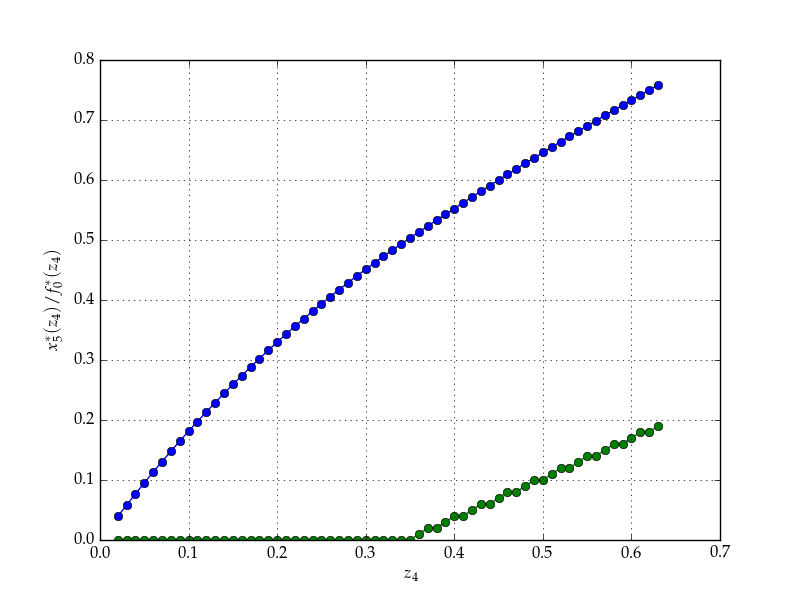
\includegraphics[width=0.8\linewidth]{opts_5}}
  \caption{Пятый шаг: зависимость  $x^*_5(z_4)$ и функция $ f^*_5(z_4) $\label{figure:opts_5}}
\end{figure}

\begin{figure}[h!]
  \label{figure:family_5}
  \center{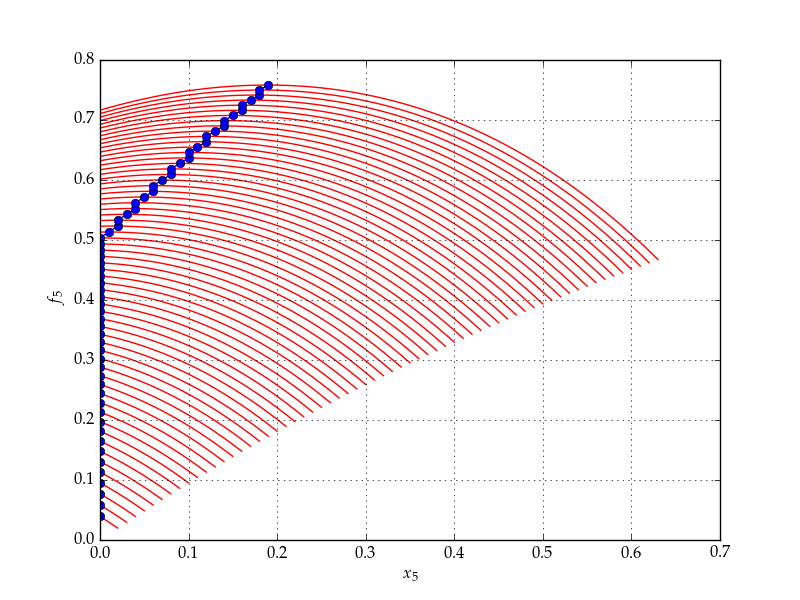
\includegraphics[width=0.8\linewidth]{family_5}}
  \caption{Пятый шаг: значения $f_{5}(x_5)$}
\end{figure}

Перейдём к оптимизации на четвёртом шаге: найдём оптимальные соотношения для вклада средств. Запас средств после третьего шага может изменяться. Наибольшее значение $ z_3 $ будет достигнуто, если все средства вложить в первый цех. Наименьший запас $ z_3 $ средств соответствует случаю, когда все средства на трёх шагах вкладывались во второй цех:

\begin{equation}
  \begin{aligned}
    z_{3,max} &= z \cdot 0,75^3 = 2 \cdot 0,75^3 = 0,844, \\
    z_{3,min} &= z \cdot 0,3^3 = 0,054.  
  \end{aligned}
\end{equation}

Рассмотрим теперь набор значений $z_3$ от $0,1$ до $0,8$ с шагом $0,1$ и для каждого значения $z_3$ найдём условное оптимальное управление на шаге $4$ и условный оптимальный доход на двух последних шагах $ f^*_{45}(z_3) $. Для этого построим серию кривых, отражающих выигрыш на двух последних шагах при любом управлении на четвёртом и при оптимальном на пятом шаге:
\begin{equation}
  \begin{aligned}
    &f_{45} = f_4(z_3, x_4) + f^*_5(z_4) = f_4(z_3, x_4) + f^*_5[0,75 \cdot x_4 + 0,3 (z_3 - x_4)], \\
    &f_4(z_3, x_4) = 2 - [e^{-x_4} + e^{-2(z_3 - x_4)}].
  \end{aligned}
\end{equation}

\begin{figure}[h!]
  \center{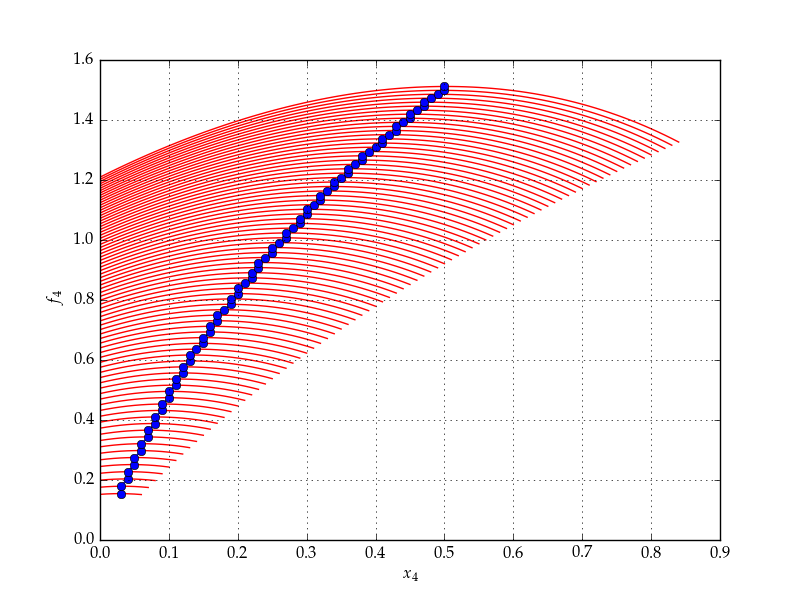
\includegraphics[width=0.85\linewidth]{family_4}}
  \caption{Четвёртый шаг: значения $f_{45}(x_4)$\label{figure:family_4}}
\end{figure}

Значения $f_{45}(x_4)$ представлены на рисунке~\ref{figure:family_4}. Для каждого значения $z_3$ максимальная ордината определяет выигрыш на двух последних шагах $f^*_{45}(z_{43})$, а абсцисса --- условное оптимальное управление $x^*_4(z_3)$. На рисунке~\ref{figure:opts_4} приведены графики зависимостей $f^*_{45}(z_3)$ и $x^*_4(z_3)$. 

\begin{figure}[h!]
  \center{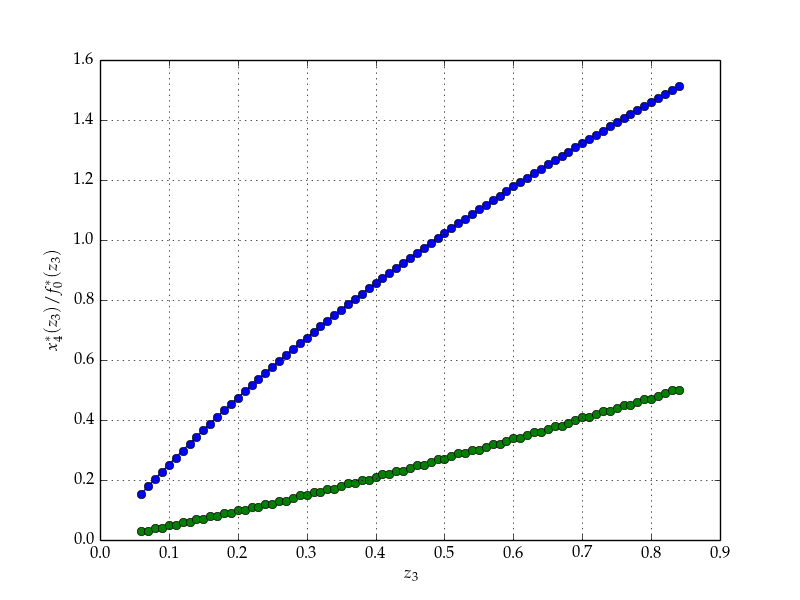
\includegraphics[width=0.85\linewidth]{opts_4}}
  \caption{Четвёртый шаг: зависимость  $x^*_4(z_3)$ и функция $ f^*_{45}(z_3) $ \label{figure:opts_4}}
\end{figure}

\newpage

Аналогично задача решается для третьего и второго шагов. Результаты приведены на рисунках~\ref{figure:family_3}~-~\ref{figure:opts_2}.

\begin{figure}[h!]
  \center{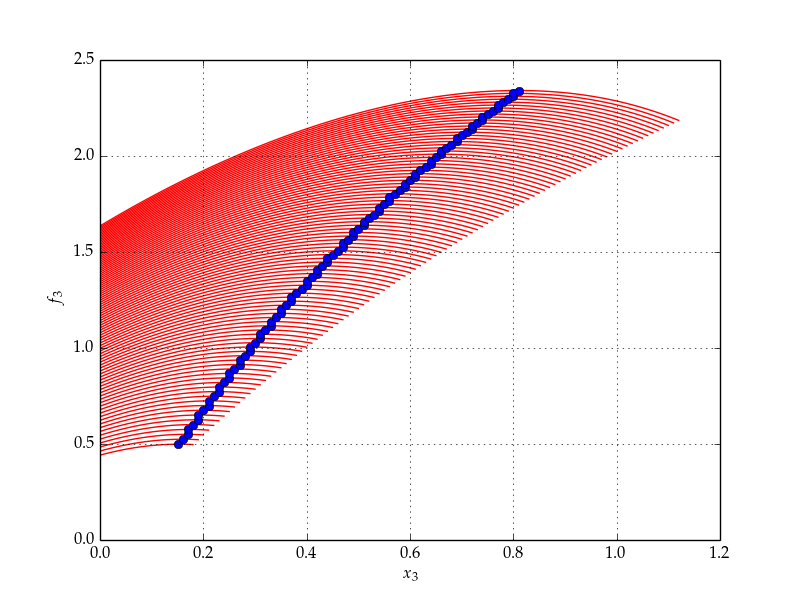
\includegraphics[width=0.8\linewidth]{family_3}}
  \caption{Третий шаг: значения $f_{345}(x_3)$\label{figure:family_3}}
\end{figure}

\begin{figure}[h!]
  \center{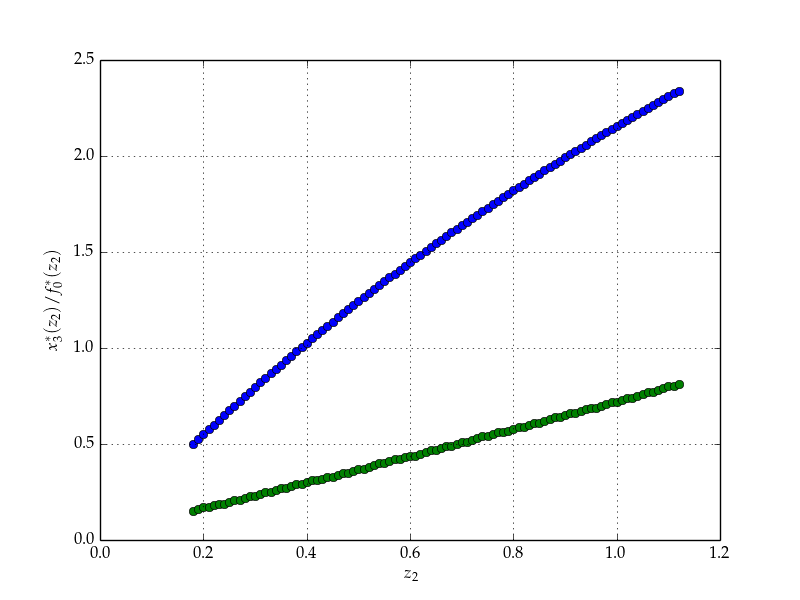
\includegraphics[width=0.8\linewidth]{opts_3}}
  \caption{Третий шаг: зависимость  $x^*_3(z_2)$ и функция $ f^*_{345}(z_2) $\label{figure:opts_3}}
\end{figure}

\begin{figure}[h!]
  \center{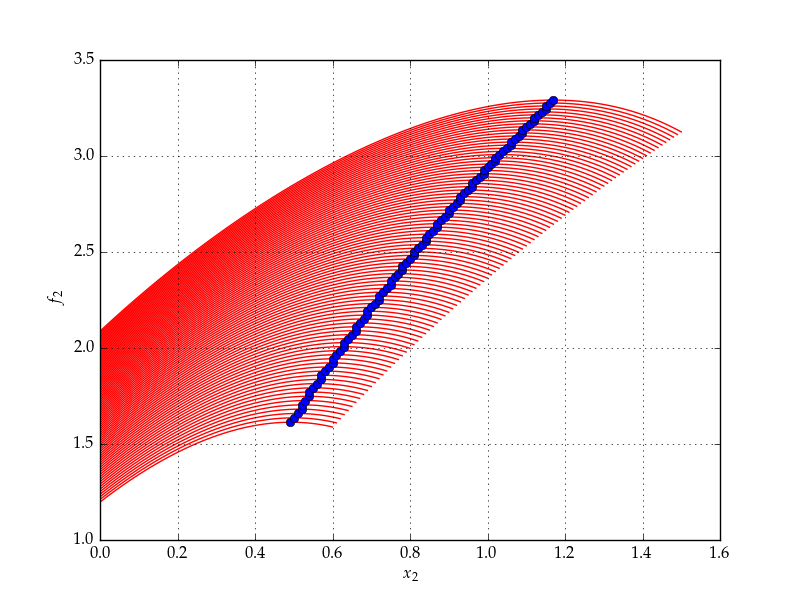
\includegraphics[width=0.85\linewidth]{family_2}}
  \caption{Второй шаг: значения $f_{2345}(x_2)$\label{figure:family_2}}
\end{figure}

\begin{figure}[h!]
  \center{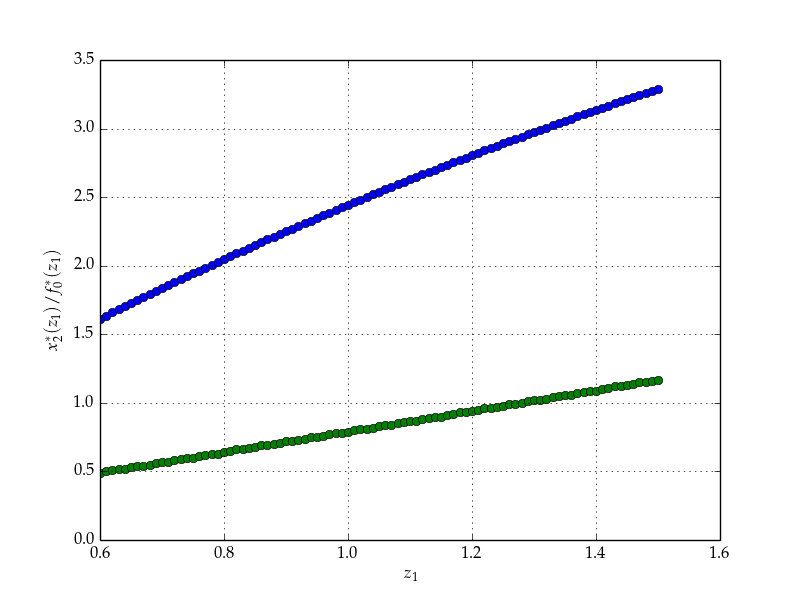
\includegraphics[width=0.85\linewidth]{opts_2}}
  \caption{Второй шаг: зависимость  $x^*_2(z_1)$ и функция $ f^*_{2345}(z_1) $\label{figure:opts_2}}
\end{figure}

Спланируем теперь первый шаг. При любом управлении на данном шаге и оптимальном на последующих пяти шагах:

\begin{equation}
  \begin{aligned}
    x_1 &= f_1(z, x_1) + f^*_{2345}(z_1) = 2-[e^{-x_1} + e^{-2(z-x_1)}] + f^*_{2345}, \\
    z_1 &= 0,75 \cdot x_1 + 0,3 (z - x_1).
  \end{aligned}
\end{equation}

На первом шаге имеющиеся ресурсы известны из условия задачи ($z =2$). Поэтому $f_{12345}(x_1)$ можно описать одной линией и соответствующее ему оптимальное управление (решение) $x^*_1 = 1.5900$. Максимальный выигрыш на первом шаге: $f_{12345} = 4.3138$.

\begin{figure}[h!]
  \center{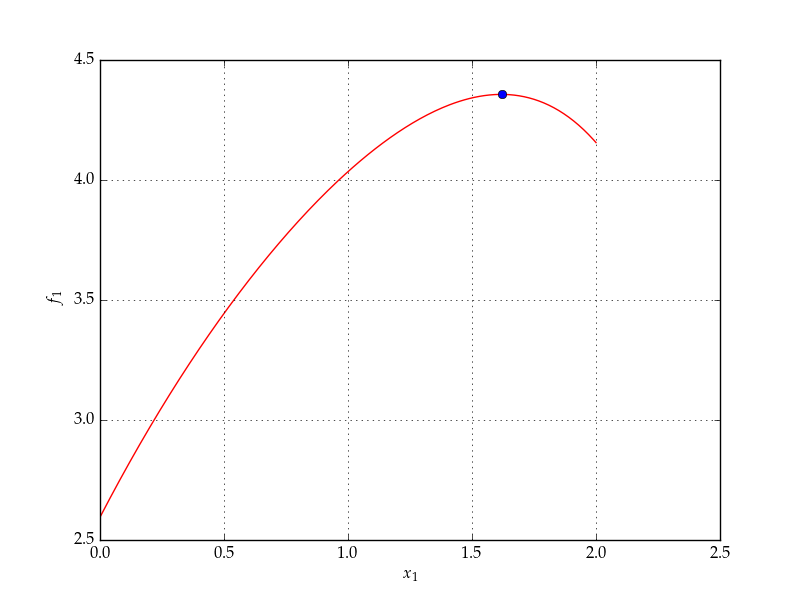
\includegraphics[width=0.9\linewidth]{family_1}}
  \caption{Первый шаг: значение $f_{12345}(x_1)$\label{figure:family_1}}
\end{figure}

\begin{figure}[h!]
  \center{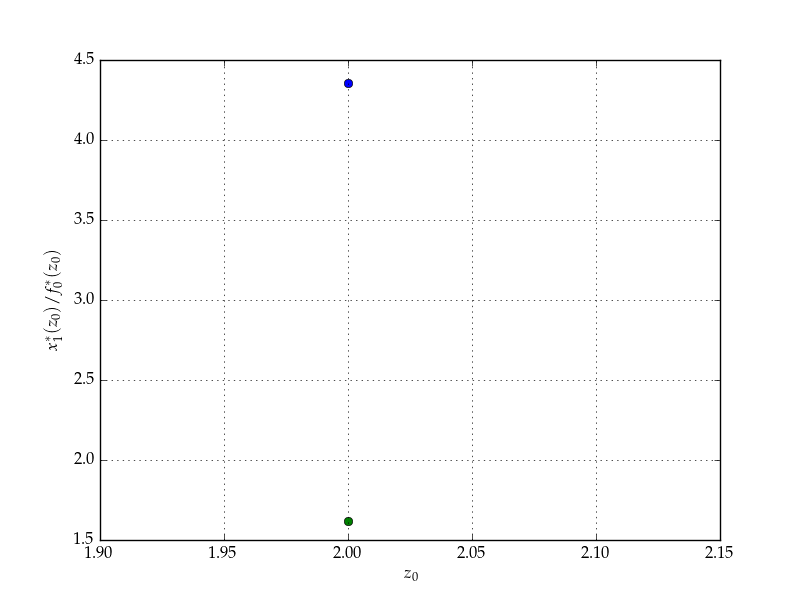
\includegraphics[width=0.85\linewidth]{opts_1}}
  \caption{Первый шаг: зависимость  $x^*_1(z_0)$ и функция $ f^*_{12345}(z_0) $\label{figure:opts_1}}
\end{figure}

\newpage

По известному оптимальному управлению на первом шаге мы можем определить запас средств к концу этого шага, что определит оптимальное управление (решение) на следующем шаге:

\begin{equation}
  z^*_1 = 0,75 x^*_1 + 0,3 (z - x^*_1) = 1.3155.
\end{equation} 

Тогда оптимальное управление на втором шаге: $x^*_2 = 1.0300$. Остаток средств к концу второго шага:

\begin{equation}
  z^*_2 = 0,75 x^*_2 + 0,3 (z - x^*_2) = 0.8582.
\end{equation}

Аналогично получим следующие значения:

\begin{equation}
  \begin{aligned}
    &x^*_3 = 0.6200, \\
    &z^*_3 = 0.5364,
    ~x^*_4 = 0.3000, \\
    &z^*_4 = 0.2959,
    ~x^*_5 = 0.
  \end{aligned}
\end{equation}

Далее получим оптимальное управление, показывающее, какое количество средств надо вкладывать в первый цех:

\begin{equation}
  \begin{aligned}
    x^*_1 &= 1.5900, \\
    x^*_2 &= 1.0300, \\
    x^*_3 &= 0.6200, \\
    x^*_4 &= 0.3000, \\
    x^*_5 &= 0.
  \end{aligned}
\end{equation}

Найдём количество средств, вкладываемых во второй цех:

\begin{equation}
  \begin{aligned}
    y^*_1 &= z - x^*_1     &= 0.4100, \\
    y^*_2 &= z^*_1 - x^*_2 &= 0.2855, \\
    y^*_3 &= z^*_2 - x^*_3 &= 0.2382, \\
    y^*_4 &= z^*_3 - x^*_4 &= 0.2364, \\
    y^*_5 &= z^*_4 - x^*_5 &= 0.2959.
  \end{aligned}
\end{equation}

Определим остаток средств: $ 0,3 \cdot 0.2959 \approx 0,09 $.

\newpage